This chapter will review some important considerations when designing and implementing a virtual reality application using gesture recognition as input method.

\section{Virtual Reality demands}
As described in the previous chapter, a virtual reality head-mounted device (HMD) is in simple terms and device that is fastened to the user's head and, when fastened, covers the
user's entire field of vision. Each eye has its own display, and both of these are positioned about 2-3 centimeters from the eyes. In addition to this several head motion
tracking sensors are built into the headset to detect any movement~\citep{POLYGON2016}. This usually includes a gyroscope, which is responsible for measuring the orientation of the
HMD, and some times an accelerometer to measure the proper acceleration of the HMD \citep{THEVERGE2016}. In addition, or instead of this, the first consumer versions of 
virtual reality headset also usually utilizes some other sensors or cameras outside the HMD. As an example the Oculus Rift CV1 utilizes constellation sensors~\cite{VRFOCUS2015}, 
which are usually positioned on a table, while the HTC Vive utilizes two "lighthouse stations", which are usually placed in opposite corners of the room, and uses photosensors and 
structured light lasers to obtain the users position and rotation~\cite{GIZMODO2015}. 
It is worth noting that both of these virtual reality headset also is sold with their own controllers, which uses similar technology as the HMD.  

\begin{figure}%[h!] %[H]
	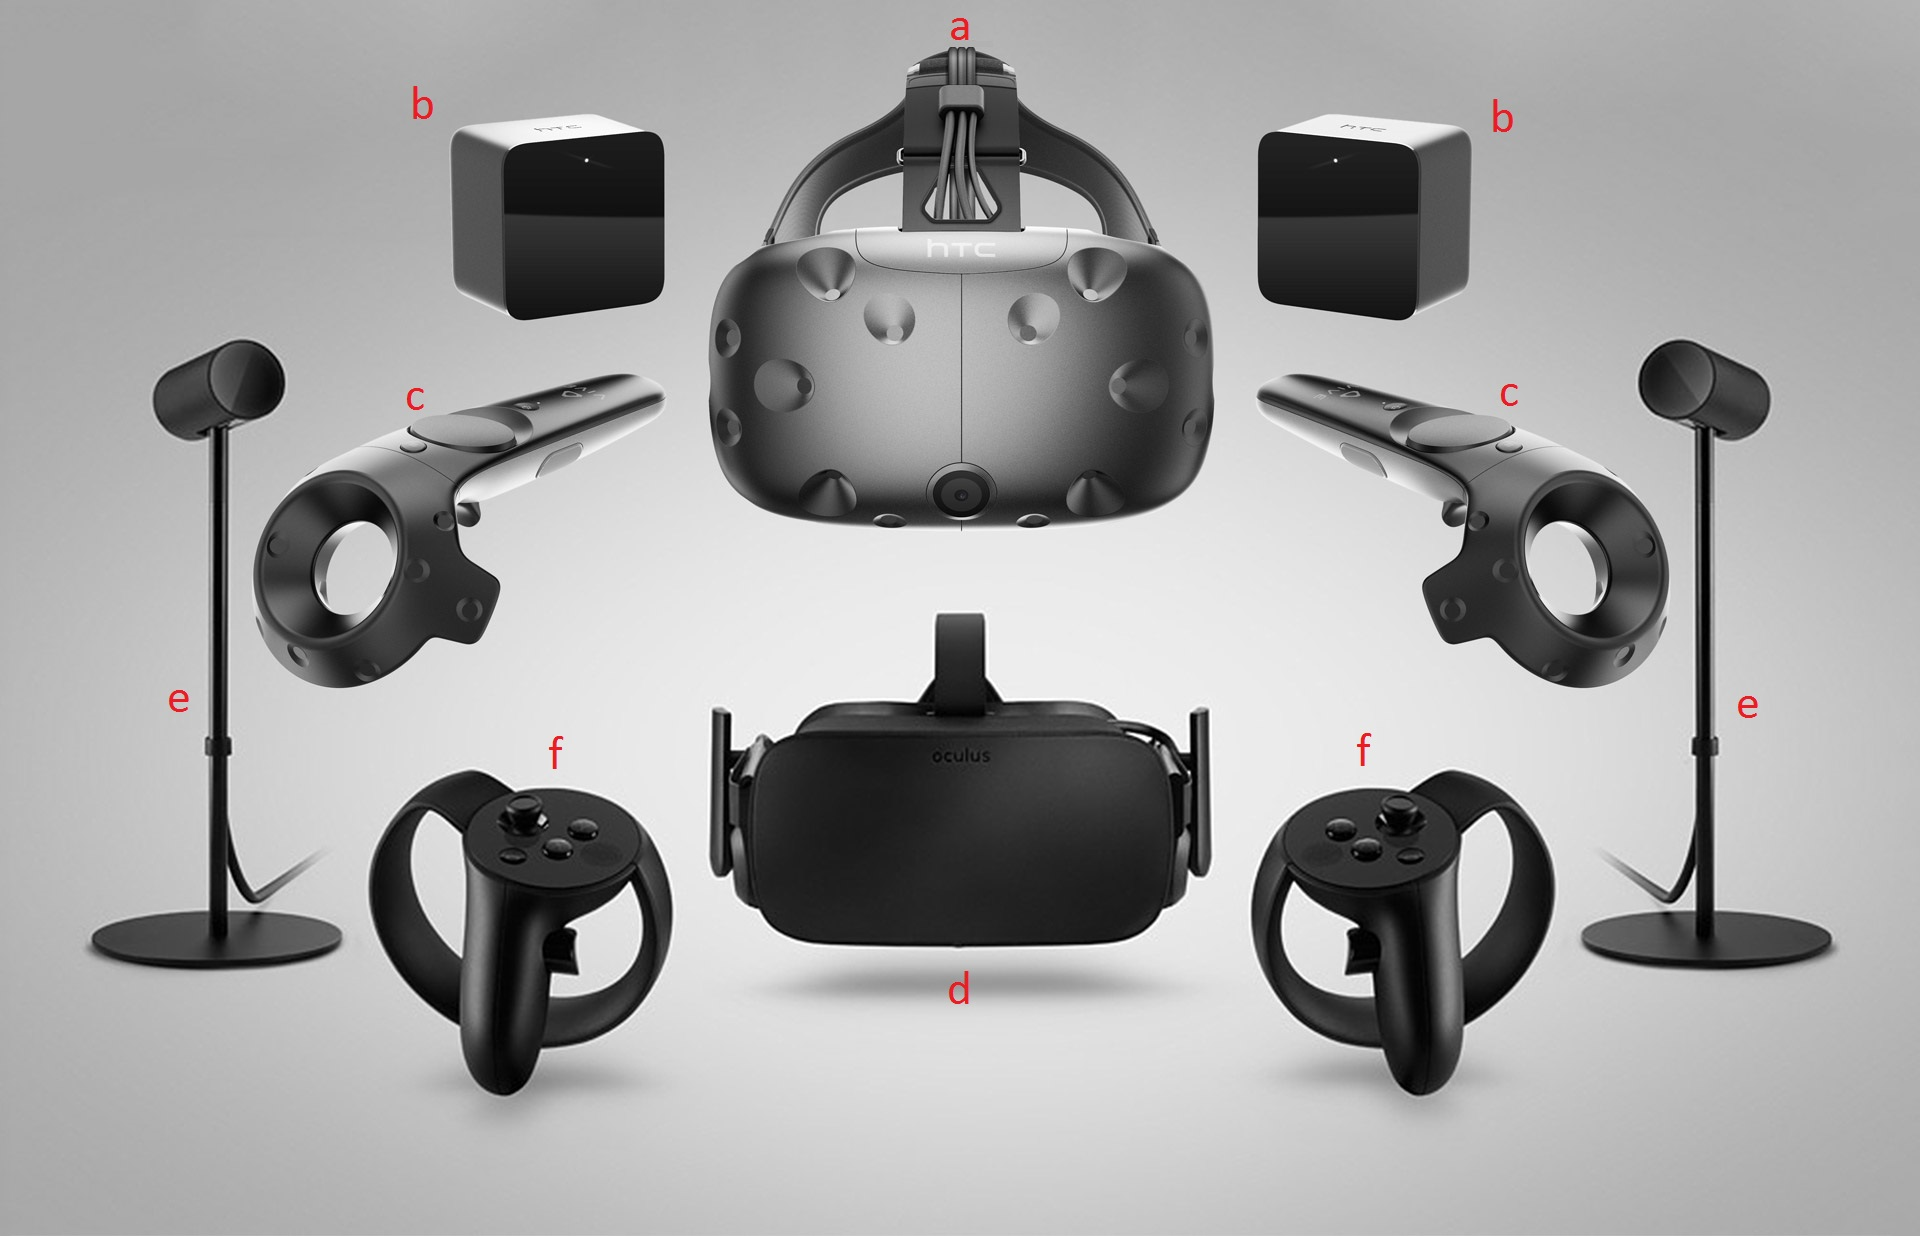
\includegraphics[width=\linewidth]{pictures/vive_and_rift_marked.jpg}
	\caption[The HTC Vive and Oculus Rift Hardware]{The HTC Vive and Oculus Rift Hardware. 
    a) The HTC Vive headset (HMD). b) The HTC Vive Lighthouse Stations. c) The HTC Vive Controllers. d) The Oculus Rift headset (HMD). e) The Oculus Rift Constellation Sensors. 
    f) The Oculus Rift Touch Controllers. Picture from \citet{ROADTOVR2016}}
	\label{fig:vive_and_rift_marked}
\end{figure} 


\section{A review of two HMD's hardware}

\subsection{The Oculus Rift CV1}

\subsection{The HTC Vive}
The HTC Vive uses more than 70 sensors \citep{BBC2015}.